% !TeX root = 01_volume_cilindro_cono_apc.tex
\begin{center}
  {\Huge \color{mainblue}\textbf{Volume e capacità cilindro}}\\[0.2cm]
  \rule{0.82\linewidth}{0.5pt}
\end{center}

\vspace{0.3cm}

\section*{1. Ricorda: Il Volume del Cilindro}

\begin{tcolorbox}[
  colback=blue!3,
  colframe=mainblue!60,
  title={Il Volume del Cilindro},
  fonttitle=\bfseries\large,
  arc=2mm,
  boxrule=1pt,
  left=5mm, right=5mm, top=3mm, bottom=3mm
]
  \begin{minipage}[c]{0.35\textwidth}
    \centering
    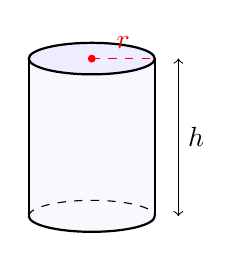
\begin{tikzpicture}[scale=1.0]
      % Cilindro liscio perfetto
      \fill[blue!5, fill opacity=0.5] (-0.8,0) -- (-0.8,2.0) arc (180:360:0.8cm and 0.2cm) -- (0.8,0) arc (360:180:0.8cm and 0.2cm);
      \filldraw[thick, fill=blue!10, fill opacity=0.7] (0,2.0) ellipse (0.8cm and 0.2cm);
      \draw[thick] (-0.8,0) -- (-0.8,2.0);
      \draw[thick] (0.8,0) -- (0.8,2.0);
      \draw[thick] (-0.8,0) arc (180:360:0.8cm and 0.2cm);
      \draw[dashed] (-0.8,0) arc (180:0:0.8cm and 0.2cm);
      
      % Raggio e quota
      \draw[dashed, red] (0,2.0) -- (0.8,2.0) node[midway, above] {$r$};
      \filldraw[red] (0,2.0) circle (1.2pt);
      \draw[<->] (1.1,0) -- (1.1,2.0) node[midway, right] {$h$};
    \end{tikzpicture}
  \end{minipage}
  \hfill
  \begin{minipage}[c]{0.55\textwidth}
    \centering
    \large
    Formula del Volume:
    \[
    V = A_b \times h = \pi \cdot r^2 \cdot h
    \]
    \vspace{0.2cm}
    \normalsize
    \begin{tabular}{rl}
      $A_b$: & Area del cerchio di base ($\pi \cdot r^2$) \\
      $r$: & Raggio della base \\
      $h$: & Altezza del cilindro
    \end{tabular}
  \end{minipage}
\end{tcolorbox}

\begin{esercizio}{La lattina di aranciata}
Una lattina cilindrica ha il raggio di base $r = 4\,\mathrm{cm}$ e l'altezza $h = 12\,\mathrm{cm}$. 

\domanda{Calcola la capacità della lattina espressa in millilitri ($\mathrm{ml}$) e centilitri ($\mathrm{cl}$).}

\responsespace{5.5cm}

\begin{soluzione}
  Passaggi:
  \begin{itemize}
    \item Volume: $V = \pi \cdot r^2 \cdot h = \pi \cdot 4^2 \times 12 = 192\pi\unita{cm^3}$.
    \item Convertiamo in capacità sapendo che $1\unita{cm^3} = 1\unita{ml}$:
    \begin{itemize}
      \item Capacità esatta: $192\pi\unita{ml}$
      \item Capacità approssimata: $C \approx 192 \times 3{,}14 \approx 602{,}88\unita{ml}$
      \item In centilitri (dividendo per $10$): $19{,}2\pi\unita{cl} \approx 60{,}288\unita{cl}$ (circa $60{,}3\unita{cl}$).
    \end{itemize}
  \end{itemize}
\end{soluzione}
\end{esercizio}

\condnewpage

\begin{esercizio}{Formula inversa del raggio}
Un serbatoio cilindrico ha un volume $V = 1600\pi\,\mathrm{cm^3}$ e un'altezza $h = 16\,\mathrm{cm}$.

\domanda{Calcola la lunghezza del raggio di base $r$.}

\responsespace{5.5cm}

\begin{soluzione}
  Passaggi:
  \begin{itemize}
    \item Dalla formula del volume $V = \pi \cdot r^2 \cdot h$, ricaviamo la formula inversa per $r^2$:
    \[
    r^2 = \frac{V}{\pi \cdot h} = \frac{1600\pi}{\pi \cdot 16} = 100\unita{cm^2}.
    \]
    \item Calcoliamo la radice quadrata per trovare $r$:
    \[
    r = \sqrt{100} = 10\unita{cm}.
    \]
  \end{itemize}
\end{soluzione}
\end{esercizio}

\condnewpage

\begin{esercizio}{Formula inversa dell'altezza}
Un bicchiere cilindrico ha il raggio di base $r = 5\,\mathrm{cm}$ e un volume totale $V = 375\pi\,\mathrm{cm^3}$.

\domanda{Se viene versato del succo d'arancia fino a riempirlo, quale altezza raggiungerà il liquido al suo interno?}

\responsespace{5.5cm}

\begin{soluzione}
  Passaggi:
  \begin{itemize}
    \item Calcoliamo prima l'area di base: $A_b = \pi \cdot r^2 = \pi \cdot 5^2 = 25\pi\unita{cm^2}$.
    \item Dalla formula del volume $V = A_b \cdot h$, ricaviamo l'altezza $h$ tramite formula inversa:
    \[
    h = \frac{V}{A_b} = \frac{375\pi}{25\pi} = 15\unita{cm}.
    \]
  \end{itemize}
\end{soluzione}
\end{esercizio}

\condnewpage

\begin{esercizio}{Il travaso proporzionale}
Una bottiglia cilindrica di raggio $r_1 = 3\,\mathrm{cm}$ e altezza $h_1 = 20\,\mathrm{cm}$ è piena d'acqua. Versiamo l'intero contenuto in un vaso cilindrico più largo, che ha un raggio di base $r_2 = 6\,\mathrm{cm}$.

\begin{center}
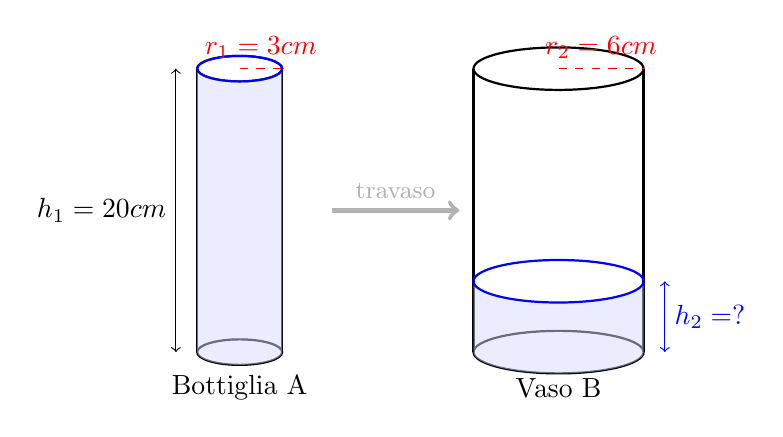
\begin{tikzpicture}[scale=0.9]
  % Cilindro 1 (Bottiglia sottile a sinistra)
  \begin{scope}[shift={(-2.5,0)}]
    \draw[thick] (0,0) ellipse (0.6cm and 0.18cm);
    \draw[thick] (-0.6,0) -- (-0.6,4.0);
    \draw[thick] (0.6,0) -- (0.6,4.0);
    \draw[thick] (0,4.0) ellipse (0.6cm and 0.18cm);
    \draw[dashed] (-0.6,0) arc (180:0:0.6cm and 0.18cm);
    
    % Acqua (pieno fino a 4.0)
    \fill[blue!15, opacity=0.5] (-0.6,0) -- (-0.6,4.0) arc (180:360:0.6cm and 0.18cm) -- (0.6,0) arc (360:180:0.6cm and 0.18cm);
    \draw[blue, thick] (0,4.0) ellipse (0.6cm and 0.18cm);
    
    % Quote
    \draw[dashed, red] (0,4.0) -- (0.6,4.0) node[midway, above] {$r_1=3\unita{cm}$};
    \draw[<->] (-0.9,0) -- (-0.9,4.0) node[midway, left] {$h_1=20\unita{cm}$};
    \node at (0, -0.5) {Bottiglia A};
  \end{scope}

  % Freccia travaso
  \draw[->, ultra thick, gray!60] (-1.2, 2.0) -- (0.6, 2.0) node[midway, above] {\small travaso};

  % Cilindro 2 (Vaso largo a destra)
  \begin{scope}[shift={(2.0,0)}]
    \draw[thick] (0,0) ellipse (1.2cm and 0.3cm);
    \draw[thick] (-1.2,0) -- (-1.2,4.0);
    \draw[thick] (1.2,0) -- (1.2,4.0);
    \draw[thick] (0,4.0) ellipse (1.2cm and 0.3cm);
    \draw[dashed] (-1.2,0) arc (180:0:1.2cm and 0.3cm);
    
    % Acqua (fino a h2 = 1.0)
    \fill[blue!15, opacity=0.5] (-1.2,0) -- (-1.2,1.0) arc (180:360:1.2cm and 0.3cm) -- (1.2,0) arc (360:180:1.2cm and 0.3cm);
    \draw[blue, thick] (0,1.0) ellipse (1.2cm and 0.3cm);
    \draw[blue, dashed] (-1.2,1.0) arc (180:0:1.2cm and 0.3cm);
    
    % Quote
    \draw[dashed, red] (0,4.0) -- (1.2,4.0) node[midway, above] {$r_2=6\unita{cm}$};
    \draw[<->, blue] (1.5,0) -- (1.5,1.0) node[midway, right] {$h_2 = ?$};
    \node at (0, -0.5) {Vaso B};
  \end{scope}
\end{tikzpicture}
\end{center}

\domanda{Quale altezza raggiungerà l'acqua nel secondo vaso?}

\responsespace{5.5cm}

\begin{soluzione}
  Passaggi:
  \begin{itemize}
    \item Calcoliamo il volume d'acqua nella prima bottiglia:
    \[
    V = \pi \cdot r_1^2 \cdot h_1 = \pi \cdot 3^2 \times 20 = 180\pi\unita{cm^3}.
    \]
    \item Calcoliamo l'area di base del secondo vaso:
    \[
    A_{b,2} = \pi \cdot r_2^2 = \pi \cdot 6^2 = 36\pi\unita{cm^2}.
    \]
    \item Troviamo l'altezza raggiunta nel secondo vaso con la formula inversa:
    \[
    h_2 = \frac{V}{A_{b,2}} = \frac{180\pi}{36\pi} = 5\unita{cm}.
    \]
    \item \textbf{Ragionamento rapido (e perché funziona):} 
    Possiamo risolvere questo esercizio all'istante capendo il legame di proporzionalità tra le grandezze:
    \begin{itemize}
      \item Il volume dell'acqua è costante: $V = A_{b,1} \times h_1 = A_{b,2} \times h_2$. Questo significa che \textbf{l'altezza e l'area di base sono inversamente proporzionali} (se l'area raddoppia, l'altezza si dimezza per mantenere lo stesso volume).
      \item L'area del cerchio dipende dal quadrato del raggio ($A_b = \pi \cdot r^2$). Se il raggio del secondo vaso è \textbf{il doppio} del primo ($3\,\mathrm{cm} \to 6\,\mathrm{cm}$), la sua area di base diventa $2^2 = 4$ \textbf{volte più grande} ($3^2 \to 6^2$).
      \item Di conseguenza, dovendo distribuire lo stesso volume su una base 4 volte più grande, l'altezza dell'acqua deve ridursi a \textbf{un quarto} del livello iniziale:
      \[
      h_2 = \frac{h_1}{4} = \frac{20\,\mathrm{cm}}{4} = 5\,\mathrm{cm}
      \]
    \end{itemize}
  \end{itemize}
\end{soluzione}
\end{esercizio}

\condnewpage

\begin{esercizio}{Archimede nel cilindro}
Un cilindro graduato ha raggio interno $r = 10\,\mathrm{cm}$ ed è parzialmente pieno d'acqua. Si immerge completamente al suo interno un blocco di metallo a forma di parallelepipedo rettangolo di dimensioni $12\,\mathrm{cm} \times 5\,\mathrm{cm} \times 8\,\mathrm{cm}$.

\domanda{Di quanti centimetri sale il livello dell'acqua ($\Delta h$) all'interno del cilindro?}

\begin{center}
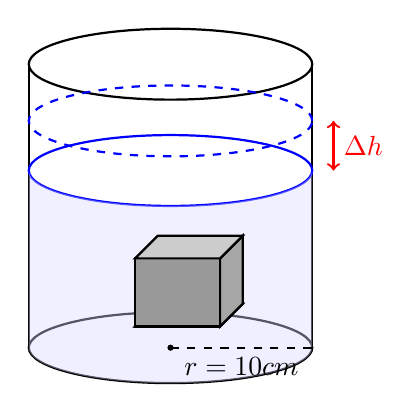
\begin{tikzpicture}[scale=0.9]
  % Cilindro esterno
  \draw[thick, fill=blue!2, fill opacity=0.3] (0,0) ellipse (2cm and 0.5cm);
  \draw[thick] (-2,0) -- (-2,4);
  \draw[thick] (2,0) -- (2,4);
  \draw[thick] (0,4) ellipse (2cm and 0.5cm);
  \draw[dashed] (-2,0) arc (180:0:2cm and 0.5cm);

  % Livello iniziale acqua (h = 2.5)
  \draw[blue, thick] (0,2.5) ellipse (2cm and 0.5cm);
  \fill[blue!15, opacity=0.4] (-2,0) -- (-2,2.5) arc (180:360:2cm and 0.5cm) -- (2,0) arc (360:180:2cm and 0.5cm);
  
  % Oggetto metallico sommerso
  \begin{scope}[shift={(-0.5,0.3)}, scale=0.8]
    \draw[thick, fill=gray!60] (0,0) -- (1.5,0) -- (1.9,0.4) -- (0.4,0.4) -- cycle;
    \draw[thick, fill=gray!80] (0,0) rectangle (1.5,1.2);
    \draw[thick, fill=gray!70] (1.5,0) -- (1.5,1.2) -- (1.9,1.6) -- (1.9,0.4) -- cycle;
    \draw[thick, fill=gray!40] (0,1.2) -- (1.5,1.2) -- (1.9,1.6) -- (0.4,1.6) -- cycle;
  \end{scope}

  % Livello finale acqua (h = 3.2)
  \draw[blue, thick, dashed] (0,3.2) ellipse (2cm and 0.5cm);
  \draw[<->, red, thick] (2.3, 2.5) -- (2.3, 3.2) node[midway, right] {$\Delta h$};

  % Quote
  \draw[dashed, thick] (0,0) -- (2,0) node[midway, below] {$r = 10\unita{cm}$};
  \filldraw (0,0) circle (1pt);
\end{tikzpicture}
\end{center}

\responsespace{5.5cm}

\begin{soluzione}
  Passaggi:
  \begin{itemize}
    \item Volume del blocco metallico: $V_{\text{blocco}} = 12 \times 5 \times 8 = 480\unita{cm^3}$.
    \item Area di base del cilindro: $A_b = \pi \cdot r^2 = \pi \cdot 10^2 = 100\pi\unita{cm^2}$.
    \item Il volume dell'acqua spostata (che ha forma cilindrica) è uguale a quello del blocco: $A_b \cdot \Delta h = V_{\text{blocco}}$.
    \[
    \Delta h = \frac{V_{\text{blocco}}}{A_b} = \frac{480}{100\pi} = \frac{4{,}8}{\pi}\unita{cm} \approx \frac{4{,}8}{3{,}14} \approx 1{,}53\unita{cm}.
    \]
  \end{itemize}
\end{soluzione}
\end{esercizio}

\condnewpage

\begin{esercizio}{La bottiglia a due cilindri}
Una bottiglia di profumo è composta da due cilindri sovrapposti:
\begin{itemize}
  \item Il Cilindro A (la base inferiore) ha raggio $R = 5\,\mathrm{cm}$ e altezza $H = 10\,\mathrm{cm}$.
  \item Il Cilindro B (il collo superiore) ha raggio $r = 2\,\mathrm{cm}$ e altezza $h = 5\,\mathrm{cm}$.
\end{itemize}

\domanda{Se versiamo nella bottiglia $266\pi\,\mathrm{ml}$ di profumo liquido, quale altezza totale (dal fondo della bottiglia) raggiungerà il liquido?}

\begin{center}
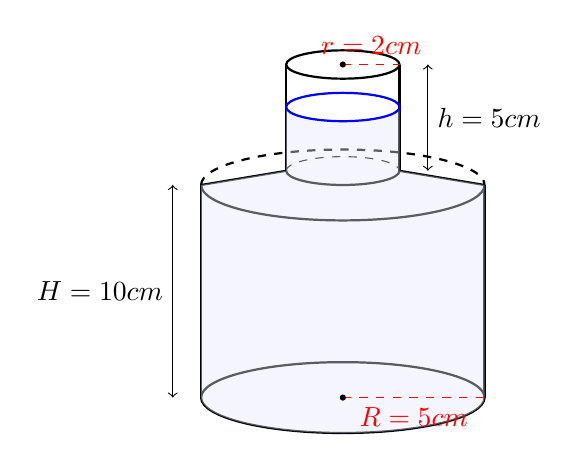
\begin{tikzpicture}[scale=0.9]
  % Cilindro Base
  \draw[thick] (0,0) ellipse (2cm and 0.5cm);
  \draw[thick] (-2,0) -- (-2,3);
  \draw[thick] (2,0) -- (2,3);
  \draw[thick] (-2,3) arc (180:360:2cm and 0.5cm);
  \draw[thick, dashed] (-2,3) arc (180:0:2cm and 0.5cm);
  \draw[dashed] (-2,0) arc (180:0:2cm and 0.5cm);
  
  % Spalle
  \draw[thick] (-2,3) -- (-0.8,3.2);
  \draw[thick] (2,3) -- (0.8,3.2);
  
  % Cilindro Collo
  \draw[thick] (-0.8,3.2) -- (-0.8,4.7);
  \draw[thick] (0.8,3.2) -- (0.8,4.7);
  \draw[thick] (0,4.7) ellipse (0.8cm and 0.2cm);
  \draw[dashed] (-0.8,3.2) arc (180:0:0.8cm and 0.2cm);
  \draw[thick] (-0.8,3.2) arc (180:360:0.8cm and 0.2cm);

  % Riempimento profumo
  \fill[blue!10, opacity=0.4] (-2,0) -- (-2,3) -- (-0.8,3.2) -- (-0.8,4.1) arc (180:360:0.8cm and 0.2cm) -- (0.8,3.2) -- (2,3) -- (2,0) arc (360:180:2cm and 0.5cm);
  \draw[blue, thick] (0,4.1) ellipse (0.8cm and 0.2cm);

  % Quote
  \draw[<->] (-2.4,0) -- (-2.4,3) node[midway, left] {$H = 10\unita{cm}$};
  \draw[<->] (1.2,3.2) -- (1.2,4.7) node[midway, right] {$h = 5\unita{cm}$};
  \draw[dashed, red] (0,0) -- (2,0) node[midway, below] {$R = 5\unita{cm}$};
  \draw[dashed, red] (0,4.7) -- (0.8,4.7) node[midway, above] {$r = 2\unita{cm}$};
  \filldraw (0,0) circle (1pt);
  \filldraw (0,4.7) circle (1pt);
\end{tikzpicture}
\end{center}

\responsespace{5.5cm}

\begin{soluzione}
  Passaggi:
  \begin{itemize}
    \item Capacità massima del Cilindro A (base): $V_{A,\text{max}} = \pi \cdot R^2 \cdot H = \pi \cdot 5^2 \cdot 10 = 250\pi\unita{cm^3} = 250\pi\unita{ml}$.
    \item Poiché il volume totale di profumo ($266\pi\unita{ml}$) è maggiore di $250\pi\unita{ml}$, il liquido riempie completamente il Cilindro A ed entra nel Cilindro B (collo).
    \item Volume di profumo residuo che sale nel Cilindro B: $V_B = 266\pi - 250\pi = 16\pi\unita{ml} = 16\pi\unita{cm^3}$.
    \item Area di base del Cilindro B: $A_{b,B} = \pi \cdot r^2 = \pi \cdot 2^2 = 4\pi\unita{cm^2}$.
    \item Altezza raggiunta all'interno del solo Cilindro B: $h_B = V_B / A_{b,B} = 16\pi / 4\pi = 4\unita{cm}$.
    \item Altezza totale a partire dal fondo della bottiglia: $h_{\text{totale}} = H + h_B = 10\unita{cm} + 4\unita{cm} = 14\unita{cm}$.
  \end{itemize}
\end{soluzione}
\end{esercizio}

\condnewpage

\section*{2. Il Volume del Cono}

\textbf{Rifletti e Ragiona:}
Pensa a un cilindro e a un cono che hanno lo stesso raggio di base e la stessa altezza (come vedi nel disegno sotto). Immagina di riempire il cono d'acqua e di versarlo nel cilindro. Noterai che servono esattamente tre travasi completi dal cono per riempire tutto il cilindro.

\begin{enumerate}[label=\alph*)]
  \item Sapendo questo, scrivi la formula per calcolare il volume del cono a partire da quello del cilindro.
\end{enumerate}

\responsespace{3cm}

\begin{soluzione}
  Ragionamento:
  Poiché il cilindro contiene esattamente 3 volte il volume del cono con stessa base e altezza, il volume del cono si calcola dividendo per 3 il volume del cilindro corrispondente:
  \[
  V_{\text{cono}} = \frac{A_b \times h}{3} = \frac{\pi \cdot r^2 \cdot h}{3}
  \]
\end{soluzione}

\begin{center}
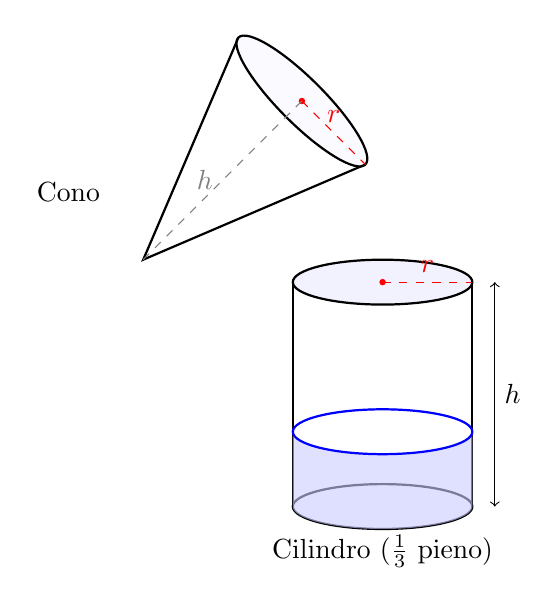
\begin{tikzpicture}[scale=0.95]
  % Cilindro a destra
  \draw[thick, fill=blue!5, fill opacity=0.3] (2,0) ellipse (1.2cm and 0.3cm);
  \draw[thick] (0.8,0) -- (0.8,3);
  \draw[thick] (3.2,0) -- (3.2,3);
  \draw[thick, fill=blue!10, fill opacity=0.5] (2,3) ellipse (1.2cm and 0.3cm);
  \draw[dashed] (0.8,0) arc (180:0:1.2cm and 0.3cm);
  
  % Acqua parziale nel cilindro (1/3 di altezza, cioè h=1)
  \fill[blue!20, opacity=0.6] (0.8,0) -- (0.8,1) arc (180:360:1.2cm and 0.3cm) -- (3.2,0) arc (360:180:1.2cm and 0.3cm);
  \draw[blue, thick] (2,1) ellipse (1.2cm and 0.3cm);
  \draw[blue, dashed] (0.8,1) arc (180:0:1.2cm and 0.3cm);
  
  % Raggio e altezza del cilindro
  \draw[dashed, red] (2,3) -- (3.2,3) node[midway, above] {$r$};
  \filldraw[red] (2,3) circle (1pt);
  \draw[<->] (3.5,0) -- (3.5,3) node[midway, right] {$h$};

  % Cono inclinato a sinistra (stessa base r=1.2, stessa altezza h=3)
  \begin{scope}[shift={(-1.2,3.3)}, rotate=-45]
    \draw[thick] (-1.2,3.0) -- (0,0) -- (1.2,3.0);
    \draw[thick, fill=blue!5, fill opacity=0.3] (0,3.0) ellipse (1.2cm and 0.3cm);
    
    % Raggio e altezza nel cono
    \draw[dashed, red] (0,3.0) -- (1.2,3.0) node[midway, above] {$r$};
    \filldraw[red] (0,3.0) circle (1pt);
    \draw[dashed, gray] (0,0) -- (0,3.0) node[midway, left] {$h$};
  \end{scope}
  
  % Labels
  \node at (2, -0.6) {Cilindro ($\frac{1}{3}$ pieno)};
  \node at (-2.2, 4.2) {Cono};
\end{tikzpicture}
\end{center}


\condnewpage

\begin{esercizio}{Applicazione con la formula del cono}
Un cono ha il raggio di base $r = 6\,\mathrm{cm}$ e l'altezza $h = 10\,\mathrm{cm}$.

\domanda{Calcola il suo volume in $\mathrm{cm^3}$.}

\responsespace{5.5cm}

\begin{soluzione}
  Passaggi:
  \begin{itemize}
    \item Calcoliamo il volume: $V = \frac{1}{3} \pi \cdot r^2 \cdot h = \frac{1}{3} \pi \cdot 6^2 \cdot 10 = \frac{1}{3} \pi \cdot 36 \cdot 10 = 120\pi\unita{cm^3}$.
    \item Valore approssimato: $V \approx 120 \times 3{,}14 \approx 376{,}8\unita{cm^3}$.
  \end{itemize}
\end{soluzione}
\end{esercizio}

\condnewpage

\begin{esercizio}{Formula inversa dell'altezza del cono}
Un cono ha l'area della base $A_b = 36\pi\,\mathrm{cm^2}$ e il volume $V = 120\pi\,\mathrm{cm^3}$.

\domanda{Calcola la sua altezza $h$.}

\responsespace{5.5cm}

\begin{soluzione}
  Passaggi:
  \begin{itemize}
    \item Sappiamo che $V = \frac{1}{3} A_b \cdot h$. Usando la formula inversa:
    \[
    h = \frac{3 \cdot V}{A_b} = \frac{3 \cdot 120\pi}{36\pi} = \frac{360\pi}{36\pi} = 10\unita{cm}.
    \]
  \end{itemize}
\end{soluzione}
\end{esercizio}

\condnewpage

\begin{esercizio}{Formula inversa del raggio del cono}
Un cono ha un'altezza $h = 9\,\mathrm{cm}$ e un volume totale $V = 108\pi\,\mathrm{cm^3}$.

\domanda{Calcola il raggio di base $r$ del cono.}

\responsespace{5.5cm}

\begin{soluzione}
  Passaggi:
  \begin{itemize}
    \item Dalla formula del volume $V = \frac{1}{3} \pi \cdot r^2 \cdot h$, sostituiamo i valori noti:
    \[
    108\pi = \frac{1}{3} \pi \cdot r^2 \times 9 \implies 108\pi = 3\pi \cdot r^2.
    \]
    \item Isoliamo $r^2$ dividendo entrambi i membri per $3\pi$:
    \[
    r^2 = \frac{108\pi}{3\pi} = 36\unita{cm^2}.
    \]
    \item Troviamo il raggio calcolando la radice quadrata:
    \[
    r = \sqrt{36} = 6\unita{cm}.
    \]
  \end{itemize}
\end{soluzione}
\end{esercizio}

\condnewpage

\section*{3. Il Tronco di Cono}

Un \textbf{tronco di cono} (la forma tipica di un secchio) è la parte inferiore che si ottiene tagliando un cono con un piano parallelo alla sua base.

\begin{center}
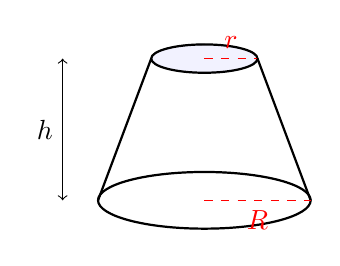
\begin{tikzpicture}[scale=0.9]
  % Base grande R=1.5
  \draw[thick] (0,0) ellipse (1.5cm and 0.4cm);
  \draw[dashed] (-1.5,0) arc (180:0:1.5cm and 0.4cm);
  
  % Sezione piccola r=0.75 a y=2
  \draw[thick, fill=blue!10, fill opacity=0.5] (0,2) ellipse (0.75cm and 0.2cm);
  \draw[dashed] (-0.75,2) arc (180:0:0.75cm and 0.2cm);
  
  % Lati
  \draw[thick] (-1.5,0) -- (-0.75,2);
  \draw[thick] (1.5,0) -- (0.75,2);
  
  % Quote
  \draw[<->] (-2.0, 0) -- (-2.0, 2) node[midway, left] {$h$};
  \draw[dashed, red] (0,0) -- (1.5,0) node[midway, below] {$R$};
  \draw[dashed, red] (0,2) -- (0.75,2) node[midway, above] {$r$};
\end{tikzpicture}
\end{center}

\begin{enumerate}[label=\alph*)]
  \item Immagina di poter conoscere qualsiasi dimensione lineare (come raggi di base e altezze). Cerca di spiegare: come calcoleresti il volume di questo tronco di cono?
\end{enumerate}

\responsespace{3.5cm}

\begin{soluzione}
  Strategia:
  Il volume del tronco di cono si ottiene immaginando di prolungare le pareti fino al vertice per ricreare il cono intero iniziale, e poi sottraendo il volume del cono piccolo superiore (la punta rimossa) dal volume del cono grande completo:
  \[
  V_{\text{tronco}} = V_{\text{cono grande}} - V_{\text{cono piccolo}}
  \]
\end{soluzione}

\condnewpage

\begin{esercizio}{Sottrazione diretta dei volumi}
Un solido a forma di tronco di cono è ottenuto rimuovendo da un cono grande di volume $1200\pi\,\mathrm{cm^3}$ un cono piccolo superiore di volume $450\pi\,\mathrm{cm^3}$.

\domanda{Calcola la capacità del tronco di cono espressa in litri ($\mathrm{l}$).}

\responsespace{5.5cm}

\begin{soluzione}
  Passaggi:
  \begin{itemize}
    \item Calcoliamo il volume del tronco per sottrazione: $V_{\text{tronco}} = V_{\text{grande}} - V_{\text{piccolo}} = 1200\pi - 450\pi = 750\pi\unita{cm^3}$.
    \item Calcoliamo il valore numerico approssimato: $750\pi \approx 750 \times 3{,}14 \approx 2355\unita{cm^3} = 2355\unita{ml}$.
    \item Convertiamo in litri dividendo per $1000$: $2355\unita{ml} = 2{,}355\unita{l}$ d'acqua.
  \end{itemize}
\end{soluzione}
\end{esercizio}

\condnewpage

\begin{esercizio}{La sfida del tronco di cono}
Un solido ha la forma di un tronco di cono. Per calcolare il suo volume, immaginiamo di ricostruire il cono intero originale prolungando la sua superficie laterale, per poi sottrarre il cono più piccolo superiore (la punta rimossa). I dati di questo modello geometrico sono:
\begin{itemize}
  \item Il cono grande intero di partenza ha un raggio di base $R = 12\,\mathrm{cm}$ e un'altezza $H = 30\,\mathrm{cm}$.
  \item Il cono piccolo superiore (la punta rimossa) ha un raggio di base $r = 6\,\mathrm{cm}$ e un'altezza $h = 15\,\mathrm{cm}$.
\end{itemize}

\domanda{Calcola il volume del tronco di cono in centimetri cubi ($\mathrm{cm^3}$) e la sua capacità equivalente in litri.}

\responsespace{5.5cm}

\begin{soluzione}
  Passaggi:
  \begin{itemize}
    \item Volume del cono grande: $V_{\text{grande}} = \frac{1}{3} \pi \cdot R^2 \cdot H = \frac{1}{3} \pi \cdot 12^2 \cdot 30 = \frac{1}{3} \pi \cdot 144 \cdot 30 = 1440\pi\unita{cm^3}$.
    \item Volume del cono piccolo rimosso: $V_{\text{piccolo}} = \frac{1}{3} \pi \cdot r^2 \cdot h = \frac{1}{3} \pi \cdot 6^2 \cdot 15 = \frac{1}{3} \pi \cdot 36 \cdot 15 = 180\pi\unita{cm^3}$.
    \item Volume del tronco di cono per sottrazione: $V_{\text{tronco}} = V_{\text{grande}} - V_{\text{piccolo}} = 1440\pi - 180\pi = 1260\pi\unita{cm^3}$.
    \item Convertiamo la capacità in litri (sapendo che $1\unita{cm^3} = 1\unita{ml}$):
    \[
    1260\pi \approx 1260 \times 3{,}14 = 3956{,}4\unita{cm^3} = 3{,}9564\unita{l} \approx 3{,}96\unita{l}.
    \]
  \end{itemize}
\end{soluzione}
\end{esercizio}

\condnewpage

\begin{esercizio}{Sfida Finale: Il Calice Decorativo}
Un calice da cocktail di design può essere modellato geometricamente combinando diverse forme: lo stelo e la base d'appoggio sono considerati come cilindri in vetro pieno, mentre la coppa superiore (il contenitore per i liquidi) è modellata come un cono vuoto. I dati geometrici di questo modello sono i seguenti:
\begin{itemize}
  \item La base d'appoggio è una base cilindrica sottile di raggio $R_b = 4\,\mathrm{cm}$ e altezza $h_b = 0{,}5\,\mathrm{cm}$.
  \item Lo stelo è un cilindro stretto di raggio $r_s = 1\,\mathrm{cm}$ e altezza $h_s = 6\,\mathrm{cm}$.
  \item La coppa superiore è un contenitore conico con raggio interno $R_c = 6\,\mathrm{cm}$ e altezza interna $H_c = 8\,\mathrm{cm}$.
\end{itemize}

\begin{center}
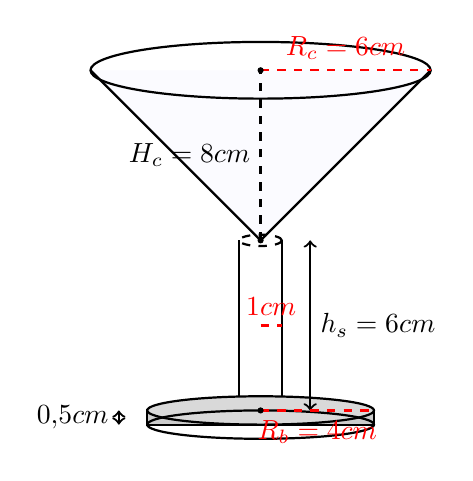
\begin{tikzpicture}[scale=0.9]
  % Coppa conica superiore
  \draw[thick, fill=blue!5, fill opacity=0.3] (-2.4,2.4) -- (0,0) -- (2.4,2.4);
  \draw[thick] (0,2.4) ellipse (2.4cm and 0.4cm);
  \draw[dashed, thick] (0,0) -- (0,2.4) node[midway, left] {$H_c = 8\unita{cm}$};
  \draw[dashed, thick, red] (0,2.4) -- (2.4,2.4) node[midway, above] {$R_c = 6\unita{cm}$};
  
  % Stelo cilindrico
  \draw[thick, fill=gray!20] (-0.3,0) -- (-0.3,-2.4);
  \draw[thick, fill=gray!20] (0.3,0) -- (0.3,-2.4);
  \draw[dashed, thick] (0.3,0) arc (0:360:0.3cm and 0.08cm);
  
  % Base d'appoggio cilindrica sottile
  \draw[thick, fill=gray!40] (-1.6,-2.4) -- (-1.6,-2.6) -- (1.6,-2.6) -- (1.6,-2.4) -- cycle;
  \draw[thick, fill=gray!30] (0,-2.4) ellipse (1.6cm and 0.2cm);
  \draw[thick] (0,-2.6) ellipse (1.6cm and 0.2cm);
  
  % Quote stelo e base
  \draw[<->, thick] (0.7,0) -- (0.7,-2.4) node[midway, right] {$h_s = 6\unita{cm}$};
  \draw[<->, thick] (-2.0,-2.4) -- (-2.0,-2.6) node[midway, left] {$0{,}5\unita{cm}$};
  \draw[dashed, thick, red] (0,-2.4) -- (1.6,-2.4) node[midway, below] {$R_b = 4\unita{cm}$};
  \draw[dashed, thick, red] (0,-1.2) -- (0.3,-1.2) node[midway, above] {$1\unita{cm}$};
  
  \filldraw (0,0) circle (1pt);
  \filldraw (0,2.4) circle (1pt);
  \filldraw (0,-2.4) circle (1pt);
\end{tikzpicture}
\end{center}

\domanda{
  \begin{enumerate}[label=\alph*)]
    \item Calcola il volume complessivo del vetro solido (stelo + base) utilizzato per fabbricare la struttura del calice.
    \item Calcola la capacità massima della coppa conica espressa in centilitri ($\mathrm{cl}$).
  \end{enumerate}
}

\responsespace{5.5cm}

\begin{soluzione}
  Passaggi:
  \begin{enumerate}[label=\alph*)]
    \item Il vetro solido è composto da due parti cilindriche:
    \begin{itemize}
      \item Base d'appoggio: cilindro con $R_b = 4\unita{cm}$ e $h_b = 0{,}5\unita{cm}$.
      \[
      V_{\text{base}} = \pi \cdot R_b^2 \cdot h_b = \pi \cdot 4^2 \times 0{,}5 = \pi \cdot 16 \times 0{,}5 = 8\pi\unita{cm^3}.
      \]
      \item Stelo: cilindro con $r_s = 1\unita{cm}$ e $h_s = 6\unita{cm}$.
      \[
      V_{\text{stelo}} = \pi \cdot r_s^2 \cdot h_s = \pi \cdot 1^2 \times 6 = 6\pi\unita{cm^3}.
      \]
      \item Volume solido totale:
      \[
      V_{\text{vetro}} = V_{\text{base}} + V_{\text{stelo}} = 8\pi + 6\pi = 14\pi\unita{cm^3} \approx 14 \times 3{,}14 \approx 43{,}96\unita{cm^3}.
      \]
    \end{itemize}
    \item Coppa conica: cono con raggio di base $R_c = 6\unita{cm}$ e altezza $H_c = 8\unita{cm}$.
    \[
    V_{\text{coppa}} = \frac{1}{3} \pi \cdot R_c^2 \cdot H_c = \frac{1}{3} \pi \cdot 6^2 \times 8 = \frac{1}{3} \pi \cdot 36 \times 8 = 96\pi\unita{cm^3}.
    \]
    Convertiamo il volume in capacità:
    \[
    96\pi\unita{cm^3} = 96\pi\unita{ml} = 9{,}6\pi\unita{cl}.
    \]
    Calcoliamo il valore numerico approssimando con $\pi \approx 3{,}14$:
    \[
    C \approx 9{,}6 \times 3{,}14 = 30{,}144\unita{cl} \approx 30{,}1\unita{cl}.
    \]
  \end{enumerate}
\end{soluzione}
\end{esercizio}
